\chapter{How To Write A Filter}
\label{chapter:WriteAFilter}

This purpose of this chapter is to assist developers create their own filter
(process object).  This chapter is divided into four major parts. An initial
definition of terms is followed by an overview of the filter creation
process. Next, data streaming is discussed, that must be understood in order
to write correct filters. Finally, a the section on multithreading describes
what you must do in order to take take advantage of shared memory parallel
processing.

\section{Terminology}
\label{sec:Terminology}

The following is some basic terminology for the discussion that follows.
Chapter \ref{chapter:SystemOverview} provides additional background
information.

\begin{itemize}
        \item The \textbf{data processing pipeline} is a directed graph of
        \textbf{process} and \textbf{data objects}. The pipeline inputs,
        operators on, and outputs data.
        \index{data processing pipeline}
        \index{process object}
        \index{data object}

        \item A \textbf{filter}, or \textbf{process object}, has one or more
        inputs, and one or more outputs.
        \index{filter}

        \item A \textbf{source}, or source process object, initiates the data
        processing pipeline, and has one or more outputs.
        \index{source}

        \item A \textbf{mapper}, or mapper process object, terminates the
        data processing pipeline. The mapper has one or more outputs, and may
        write data to disk, interface with a display system, or interface to
        any other system.
        \index{mapper}

        \item A \textbf{data object} represents and provides access to
        data. In ITK, the data object (ITK class DataObject) is typically of
        type itk::Image or itk::Mesh.
        \index{data object}

        \item A \textbf{region} (ITK class itk::Region) represents a piece,
        or subset of the entire data set.
        \index{region}

        \item An \textbf{image region} (ITK class itk::ImageRegion)
        represents a structured portion of data. ImageRegion is implemented
        using the Index and Size classes
        \index{image region}

        \item A \textbf{mesh region} (ITK class itk::MeshRegion) represents
        an unstructured portion of data.
        \index{mesh region}

        \item The \textbf{LargestPossibleRegion} is the theoretical single,
        largest piece (region) that could represent the entire dataset. The
        LargestPossibleRegion is used in the system as the measure of the
        largest possible data size.
        \index{LargestPossibleRegion}

        \item The \textbf{BufferedRegion} is a contiguous block of memory
        that is lesss than or equal to in size to the
        LargestPossibleRegion. The buffered region is what has actually been
        allocated by a filter to hold its output.
        \index{BufferedRegion}

        \item The \textbf{RequestedRegion} is the piece of the dataset that a
        filter is required to produce. The RequestedRegion is less than or
        equal in size to the BufferedRegion. The RequestedRegion may differ
        in size from the BufferedRegion due to performance reasons. The
        RequestedRegion may be set by a user, or by an application that needs
        just a portion of the data.
        \index{RequestedRegion}

        \item The \textbf{modified time} (represented by ITK class
        itk::TimeStamp) is a monotonically increasing integer value that
        characterizes a point in time when an object was last modified.
        \index{modified time}

        \item \textbf{Downstream} is the direction of dataflow, from sources
        to mappers.
        \index{pipeline!downstream}

        \item \textbf{Upstream} is the opposite of downstream, from mappers
        to sources.
        \index{pipeline!upstream}

        \item The \textbf{pipeline modified time} for a particular data
        object is the maximum modified time of all upstream data objects and
        process objects.
        \index{pipeline!modified time}

        \item The term \textbf{information} refers to metadata that
        characterizes data. For example, index and dimensions are information
        characterizing an image region.
        \index{pipeline!information}
\end{itemize}

\section{Overview of Filter Creation}
\label{sec:OverviewFilterCreation}
\index{filter!overview of creation|textbf}

Filters are defined with respect to the type of data they input (if any), and
the type of data they output (if any). The key to writing a ITK filter is to
identify the number and types of input and output. Having done so, there are
often superclasses that simplify this task via class derivation. For example,
most filters in ITK take a single image as input, and produce a single image
on output. The superclass itk::ImageToImageFilter is a convenience class that
provide most of the functionality needed for such a filter.

Once the appropriate superclass is identified, the filter writer implements
the class defining the methods required by most all ITK objects: New(),
PrintSelf, and protected constructor, copy constructor, delete, and
operator=, and so on (don't forget standard typedefs like Self, Superclass,
Pointer, and ConstPointer). Then the filter writer can focus on the most
important parts of the implementation: defining the API, data members, and
other implementation details of the algorithm. In particular, the filter
writer will have to implement either a GenerateData() (non-threaded) or
ThreadedGenerateData() method. (See ``'' for more information.)

An important note: the GenerateData() method is required to allocate memory
for the output. The ThreadedGenerateData() method is not. In default
implementation (see itk::ImageSource, a superclass of
itk::ImageToImageFilter) GenerateData() allocates memory and then invokes 
ThreadedGenerateData().

One of the most important decisions that the developer must make is whether
the filter can stream data; that is, process just a portion of the input to
produce a portion of the output. Often superclass behavior works well: if the
filter processes the input using single pixel access, then the default
behavior is adequate. If not, then the user may have to a) find a more
specialized superclass to derive from, or b) override one or more methods
that control how the filter operates during pipeline execution. The next
section describes these methods.

\begin{figure}
  \par\centering
  \resizebox{5in}{!}{ 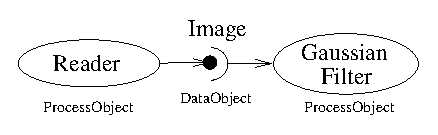
\includegraphics{DataPipelineOneConnection.eps}} 
  \caption{\label{fig:DataPipeLineOneConnection}Relationship between itk::DataObjects and itk::ProcessObjects }
  \par
\end{figure}

\section{Streaming Large Data}
\label{sec:StreamingLargeData}
\index{pipeline!streaming large data}

Image, volume, and higher-dimensional data is large and becoming larger. This
trend is due to advances in scanning resolution, as well as increases in
computing capability. Any practical segmentation and registration software
system must address this fact in order to be useful in application. ITK
addresses this problem via its data streaming facility.

In ITK, streaming is the process of dividing data into pieces, or regions,
and then processing this data through the data pipeline. Recall that the
pipeline consists of process objects that generate data objects, connected
into a pipeline topology. The input to a process object is a data object
(unless the process initiates the pipeline and then it is a source, process
object). These data objects in turn are consumed by other process objects,
and so on, until a directed graph of data flow is constructed. Eventually the
pipeline is terminated by one or more mappers, that may write data to
storage, or interface with a graphics or other system. This is illustrated in 
figures \ref{fig:DataPipeLineOneConnection} and \ref{fig:DataPipeLine}.

A significant benefit of this architecture is that the relatively complex
process of managing pipeline execution is designed into the system. This
means that keeping the pipeline up to date, executing only those portions of
the pipeline that have changed, multithreading execution, managing memory
allocation, and streaming is all built into the architecture. However, these
features do introduce complexity into the system, the bulk of which is seen
by class developers. The purpose of this chapter is to describe the pipeline
execution process in detail, with a focus on data streaming.


\subsection{Overview of Pipeline Execution}
\label{sec:OverviewPipelineExecution}
\index{pipeline!overview of execution|textbf}

The pipeline execution process performs several important functions.

\begin{figure}
  \par\centering
  \resizebox{5in}{!}{ 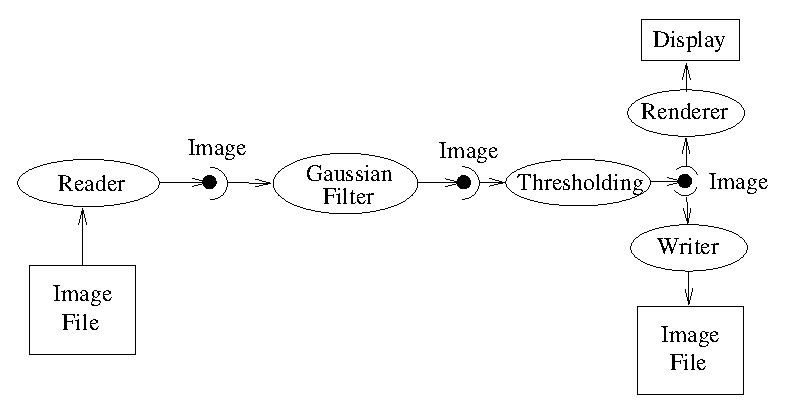
\includegraphics{DataPipeline.eps}} 
  \caption{\label{fig:DataPipeLine}The Data Pipeline}
  \par
\end{figure}

\begin{enumerate}
        \item It determines which filters, in a pipeline of filters, need to
        execute. This prevents redundant execution and minimizes overall
        execution time.

        \item It initializes the (filter's) output data objects, preparing
        them for new data.  In addition, it determines how much memory each
        filter must allocate for its output, and allocates it.

        \item The execution process determines how much data a filter must
        process in order to produce an output of sufficient size for
        downstream filters; it also takes into account any limits on memory
        or special filter requirements. Other factors include the size of
        data processing kernels, that affect how much data needs to be input
        (extra padding).

        \item It subdivides data into subpieces for multithreading. (Note
        that the division of data into subpieces is exactly same problem as
        dividing data into pieces for streaming; hence multithreading comes
        for free as part of the streaming architecture.)

        \item It may free (or release) output data if filters no longer need
        it to compute, and the user requests that data is to be
        released. (Note: a filter's output data object may be considered a
        ``cache''. If the cache is allowed to remain (ReleaseDataOff) between
        pipeline execution, and the filter, or the input to the filter, never
        changes, then process objects downstream of the filter just reuse the
        filter's cache to reexecute.)
\end{enumerate}

To perform these function, the execution process negotiates with the
filters that define the pipeline. Only each filter can know how much is data is
required on input to produce a particular output. For example, a shrink
filter with a shrink factor of two requires an image twice as large (in terms
of its x-y dimensions) on input to produce a particular size output. Or, an
image convolution filter would require extra input (boundary padding)
depending on the size of the convolution kernel. Some filters require the
entire input to produce an output (for example, a histogram), and have the
option of requesting the entire input. (In this case streaming does not work
unless the developer creates a filter that can request multiple pieces,
caching state between each piece to assemble the final output.)


\begin{figure}
  \par\centering
  \resizebox{5in}{!}{ 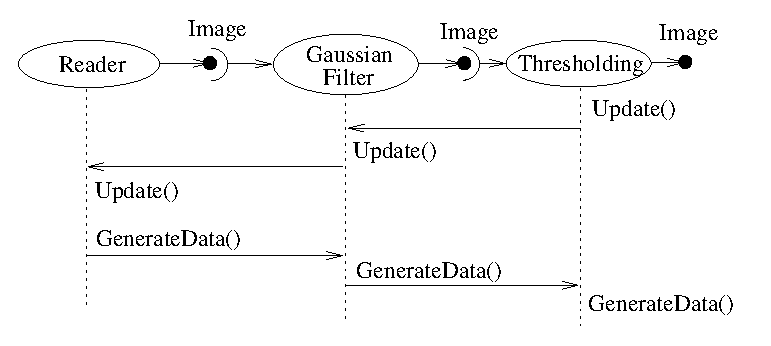
\includegraphics{DataPipelineUpdate.eps}} 
  \caption{\label{fig:DataPipeLineUpdate}Sequence of the Data Pipeline updating mechanism}
  \par
\end{figure}


Ultimately the negotiation process is controlled by the request for data of a
particular size (i.e., region). It may be that the user asks to process a
region of interest within a large image, or that memory limitations result in
processing the data in several pieces. For example, an application may
compute the memory required by a pipeline, and then use
itk::StreamingImageFilter to break the data processing into several pieces.
The data request is propagated through the pipeline in the upstream
direction, and the negotiation process configures each filter to produce
output data of a particular size.

The secret to creating a streaming filter is to understand how this
negotiation process works, and how to override its default behavior by using
the appropriate virtual functions defined in itk::ProcessObject. The next
section describes the specifics of these methods, and when to override
them. Examples are provided along the way to illustrate concepts.


\subsection{Details of Pipeline Execution}
\label{sec:DetailsPipelineExecution}
\index{pipeline!execution details|textbf}

Typically pipeline execution is initiated when a process object receives the
ProcessObject::Update() method invocation. This method is simply delegated to
the output of the filter, invoking the DataObject::Update() method. Note that
this behavior is typical of the interaction between ProcessObject and
DataObject: a method invoked on one is eventually delegated to the other. In
this way the data request from the pipeline is propagated upstream,
initiating data flow that returns downstream.

The DataObject::Update() method in turn invokes three other methods:

\begin{itemize}
        \item DataObject::UpdateOutputInformation()
        \item DataObject::PropagateRequestedRegion()
        \item DataObject::UpdateOutputData()
\end{itemize}

\subsubsection{UpdateOutputInformation()}
\label{sec:UpdateOutputInformation}
\index{pipeline!UpdateOutputInformation|textbf}

The UpdateOutputInformation() method determines the pipeline modified
time. It may set the RequestedRegion and the LargestPossibleRegion depending
on how the filters are configured. (The RequestedRegion is set to process all
the data, i.e., the LargestPossibleRegion, if it has not been set.) The
UpdateOutputInformation() propagates upstream through the entire pipeline and
terminates at the sources.

During UpdateOutputInformation(), filters have a chance to override the
ProcessObject::GenerateOutputInformation() method
(GenerateOutputInformation() is invoked by UpdateOutputInformation()). This
virtual method invokes DataObject::CopyInformation. The default behavior is
for the GenerateOutputInformation() to copy the meta data describing the
input to the output (via DataObject::CopyInformation()). Remember,
information is metadata describing the output, such as (for an image) the
origin, spacing, and LargestPossibleRegion (i.e., largest possible size) of
the image.

A good example of this behavior is itk::ShrinkImageFilter. This filter takes
an input image and shrinks it by some integral value. The result is that the
spacing and LargestPossibleRegion of the output change. Thus,
GenerateOutputInformation() is overloaded.

\subsubsection{PropagateRequestedRegion()}
\label{sec:PropagateRequestedRegion}
\index{pipeline!PropagateRequestedRegion|textbf}

The PropagateRequestedRegion() propagates upstream to satisfy a data
request. In typical application this data request is usually the
LargestPossibleRegion, but if streaming is necessary, or the user is
interested in updating just a portion of the data, the RequestedRegion may be
any valid region within the LargestPossibleRegion.

The function of PropagateRequestedRegion() is, given a request for data (the
amount is specified by RequestedRegion), propagate upstream configuring the
filter's input and output process object's to the correct size. Eventually,
this means configuring the BufferedRegion, that is the amount of data
actually allocated.

The reason for the buffered region is this: the output of a filter may be
consumed by more than one downstream filter. If these consumers each request
different amounts of input (say due to kernel requirements or other padding
needs), then the upstream, generating filter produces the data to satisfy
both consumers, that may mean it produces more data than one of the
consumers needs.

The ProcessObject::PropagateRequestedRegion() method invokes three methods
that the filter developer may choose to overload. 

\begin{itemize}
        \item EnlargeOutputRequestedRegion(DataObject *output) gives the
        (filter) subclass a chance to indicate that it will provide more data
        then required for the output. This can happen, for example, when a
        source can only produce the whole output (i.e., the
        LargestPossibleRegion).

        \item GenerateOutputRequestedRegion(DataObject *output) gives the
        subclass a chance to define how to set the requested regions for each
        of its outputs, given this output's requested region.  The default
        implementation is to make all the output requested regions the same.
        A subclass may need to override this method if each output is a
        different resolution. This method is only overridden if a filter has
        multiple outputs.

        \item GenerateInputRequestedRegion() gives the subclass a chance to
        request a larger requested region on the inputs. This is necessary
        when, for example, a filter requires more data at the "internal"
        boundaries to produce the boundary values - due to kernel operations
        or other region boundary effects.
\end{itemize}

itk::GibbsPriorFilter is an example of a filter that needs to invoke
EnlargeOutputRequestedRegion(). The designer of this filter decided that the
filter should operate on all the data. Note that a subtle interplay between
this method and GenerateInputRequestedRegion() is occurring here. The default
behavior of GenerateInputRequestedRegion (at least for
itk::ImageToImageFilter) is to set the input RequestedRegion to the output
ReqestedRegion. Hence, by overriding the EnlargeOutputRequestedRegion() to
set the output to the LargestPossibleRegion, the input to this filter is the
LargestPossibleRegion (and probably is that all upstream filters process
their LargestPossibleRegion as well. This means that the filter, and
therefore the pipeline, does not stream. This could be fixed by
reimplementing the filter with the notion of streaming built in to the
algorithm.)

itk::GradientMagnitudeImageFilter is an example of a filter that needs to
invoke GenerateInputRequestedRegion(). It needs a larger input requested
region because a kernel is required to compute the gradient at a pixel. Hence
the input needs to be ``padded out'' so the filter has enough data to compute
the gradient at each output pixel.

\subsubsection{UpdateOutputData()}
\label{sec:UpdateOutputData}
\index{pipeline!UpdateOutputData|textbf}

UpdateOutputData() is the third and final method as a result of the Update()
method. The purpose of this method is to determine whether a particular
filter needs to execute in order to bring its output up to date. (A filter
executes when its GenerateData() method is invoked.) Filter execution occurs
when a) the filter is modified as a result of modifying an instance variable;
b) the input to the filter changes; c) the input data has been released; or
d) an invalid RequestedRegion was set previously and the filter did not
produce data. Filters execute in order in the downstream direction. Once a
filter executes, all filters downstream of it must also execute.

DataObject::UpdateOutputData() is delegated to the DataObject's source (i.e.,
the ProcessObject that generated it) only if the DataObject needs to be
updated. A comparison of modified time, pipeline time, release data flag, and
valid requested region is made. If any one of these conditions indicate that
the data needs regeneration, then the source's
ProcessObject::UpdateOutputData() is invoked. These calls are made
recursively up the pipeline until a source filter object is encountered, or
the pipeline is determined to be up to date and valid. At this point, the
recursion unrolls, and the execution of the filter proceeds. (This means that
the output data is initialized, StartEvent is invoked, the filters
GenerateData() is called, EndEvent is invoked, and input data to this filter
may be released, if requested. In addition, this filter's InformationTime is
updated to the current time.)

The developer will never override UpdateOutputData(). The developer need only
write the GenerateData() method (non-threaded) or ThreadedGenerateData()
method. A discussion of threading follows in the next section.


\section{Threaded Filter Execution}
\label{sec:ThreadedFilterExecution}
\index{pipeline!ThreadedFilterExecution|textbf}

Filters that can process data in pieces can typically multi-process using the
data parallel, shared memory implementation built into the pipeline execution
process. To create a multithreaded filter, simply define and implement a
ThreadedGenerateData() method. For example, a itk::ImageToImageFilter would create the method:

\begin{verbatim}
    void ThreadedGenerateData(const OutputImageRegionType& 
                              outputRegionForThread, int threadId)
\end{verbatim}

The key to threading is to generate output for the output region given (as
the first parameter in the argument list above). In ITK, this is simple to do
because an output iterator can be created using the region provided. Hence
the output can be iterated over, accessing the corresponding input pixels as
necessary to compute the value of the output pixel.

Multi-threading requires caution when producing output or invoking
events. Normally only thread id zero is allowed to produce output or generate
events. (The threadId is passed into ThreadedGenerateData()). If more than
one thread tries to write at the same time, the program can behave badly, and
even crash.

